\documentclass[journal,12pt,twocolumn]{IEEEtran}

\usepackage{setspace}
\usepackage{gensymb}
\singlespacing
\usepackage[cmex10]{amsmath}

\usepackage{amsthm}

\usepackage{mathrsfs}
\usepackage{txfonts}
\usepackage{amsmath}
\usepackage{stfloats}
\usepackage{float} 
\usepackage{bm}
\usepackage{tikz}
\usepackage{pgfplots}
\usepackage{cite}
\usepackage{cases}
\usepackage{subfig}

\usepackage{longtable}
\usepackage{multirow}

\usepackage{enumitem}
\usepackage{mathtools}
\usepackage{steinmetz}
\usepackage{tikz}
\usepackage{circuitikz}
\usepackage{verbatim}
\usepackage{tfrupee}
\usepackage[breaklinks=true]{hyperref}
\usepackage{graphicx}
\usepackage{tkz-euclide}

\usetikzlibrary{calc,math}
\usetikzlibrary{shapes.geometric, arrows}
\usepackage{listings}
    \usepackage{color}                                            %%
    \usepackage{array}                                            %%
    \usepackage{longtable}                                        %%
    \usepackage{calc}                                             %%
    \usepackage{multirow}                                         %%
    \usepackage{hhline}                                           %%
    \usepackage{ifthen}                                           %%
    \usepackage{lscape}     
\usepackage{multicol}
\usepackage{chngcntr}
\usepackage{hyperref}
\hypersetup{
    colorlinks=true,
    linkcolor=blue,
    filecolor=blue,      
    urlcolor=blue,
}
\DeclareMathOperator*{\Res}{Res}
\DeclareMathOperator{\sinc}{sinc}

\renewcommand\thesection{\arabic{section}}
\renewcommand\thesubsection{\thesection.\arabic{subsection}}
\renewcommand\thesubsubsection{\thesubsection.\arabic{subsubsection}}

\renewcommand\thesectiondis{\arabic{section}}
\renewcommand\thesubsectiondis{\thesectiondis.\arabic{subsection}}
\renewcommand\thesubsubsectiondis{\thesubsectiondis.\arabic{subsubsection}}


\hyphenation{op-tical net-works semi-conduc-tor}
\def\inputGnumericTable{}                                 %%

\lstset{
%language=C,
frame=single, 
breaklines=true,
columns=fullflexible
}

\makeatletter
\setlength{\@fptop}{0pt}
\makeatother

\begin{document}


\newtheorem{theorem}{Theorem}[section]
\newtheorem{problem}{Problem}
\newtheorem{proposition}{Proposition}[section]
\newtheorem{lemma}{Lemma}[section]
\newtheorem{corollary}[theorem]{Corollary}
\newtheorem{example}{Example}[section]
\newtheorem{definition}[problem]{Definition}

\newcommand{\BEQA}{\begin{eqnarray}}
\newcommand{\EEQA}{\end{eqnarray}}
\newcommand{\define}{\stackrel{\triangle}{=}}
\newcommand*\Eval[3]{\left.#1\right\rvert_{#2}^{#3}}
\bibliographystyle{IEEEtran}
\raggedbottom
\setlength{\parindent}{0pt}
\providecommand{\mbf}{\mathbf}
\providecommand{\pr}[1]{\ensuremath{\Pr\left(#1\right)}}
\providecommand{\qfunc}[1]{\ensuremath{Q\left(#1\right)}}
\providecommand{\sbrak}[1]{\ensuremath{{}\left[#1\right]}}
\providecommand{\lsbrak}[1]{\ensuremath{{}\left[#1\right.}}
\providecommand{\rsbrak}[1]{\ensuremath{{}\left.#1\right]}}
\providecommand{\brak}[1]{\ensuremath{\left(#1\right)}}
\providecommand{\lbrak}[1]{\ensuremath{\left(#1\right.}}
\providecommand{\rbrak}[1]{\ensuremath{\left.#1\right)}}
\providecommand{\cbrak}[1]{\ensuremath{\left\{#1\right\}}}
\providecommand{\lcbrak}[1]{\ensuremath{\left\{#1\right.}}
\providecommand{\rcbrak}[1]{\ensuremath{\left.#1\right\}}}
\theoremstyle{remark}
\newtheorem{rem}{Remark}
\newcommand{\sgn}{\mathop{\mathrm{sgn}}}
\providecommand{\abs}[1]{$\left\vert#1\right\vert$}
\providecommand{\res}[1]{\Res\displaylimits_{#1}} 
\providecommand{\norm}[1]{$\left\lVert#1\right\rVert$}
%\providecommand{\norm}[1]{\lVert#1\rVert}
\providecommand{\mtx}[1]{\mathbf{#1}}
\providecommand{\mean}[1]{$E\left[ #1 \right]$}
\providecommand{\fourier}{\overset{\mathcal{F}}{ \rightleftharpoons}}
%\providecommand{\hilbert}{\overset{\mathcal{H}}{ \rightleftharpoons}}
\providecommand{\system}{\overset{\mathcal{H}}{ \longleftrightarrow}}
	%\newcommand{\solution}[2]{\textbf{Solution:}{#1}}
\newcommand{\solution}{\noindent \textbf{Solution: }}
\newcommand{\cosec}{\,\text{cosec}\,}
\providecommand{\dec}[2]{\ensuremath{\overset{#1}{\underset{#2}{\gtrless}}}}
\newcommand{\myvec}[1]{\ensuremath{\begin{pmatrix}#1\end{pmatrix}}}
\newcommand{\mydet}[1]{\ensuremath{\begin{vmatrix}#1\end{vmatrix}}}
\newcommand*{\permcomb}[4][0mu]{{{}^{#3}\mkern#1#2_{#4}}}
\newcommand*{\perm}[1][-3mu]{\permcomb[#1]{P}}
\newcommand*{\comb}[1][-1mu]{\permcomb[#1]{C}}
\numberwithin{equation}{subsection}
\makeatletter
\@addtoreset{figure}{problem}
\makeatother
\let\StandardTheFigure\thefigure
\let\vec\mathbf
\renewcommand{\thefigure}{\theproblem}
\def\putbox#1#2#3{\makebox[0in][l]{\makebox[#1][l]{}\raisebox{\baselineskip}[0in][0in]{\raisebox{#2}[0in][0in]{#3}}}}
     \def\rightbox#1{\makebox[0in][r]{#1}}
     \def\centbox#1{\makebox[0in]{#1}}
     \def\topbox#1{\raisebox{-\baselineskip}[0in][0in]{#1}}
     \def\midbox#1{\raisebox{-0.5\baselineskip}[0in][0in]{#1}}
\vspace{3cm}
\title{GATE Assignment 1}
\author{Perambuduri Srikaran - AI20BTECH11018}
\maketitle
\newpage
\bigskip
\renewcommand{\thefigure}{\theenumi}
\renewcommand{\thetable}{\theenumi}
%Download all python codes from
%\begin{lstlisting}
%https://github.com/srikaran-p/AI1103/tree/main/Assign%ment4/codes
%\end{lstlisting}
%and latex codes from 
Download all python codes from
\begin{lstlisting}
https://github.com/srikaran-p/AI1103/tree/main/GATEAssignment1/codes
\end{lstlisting}
Download all latex codes from 
\begin{lstlisting}
https://github.com/srikaran-p/EE3900/tree/main/GATEAssignment1
\end{lstlisting}
\section*{Problem}
(GATE EC-2018 Q.39) The input $4\sinc{\brak{2t}}$ is fed to a Hilbert transformer to obtain $y\brak{t}$, as shown in the figure below:
\tikzstyle{noborder} = [rectangle, draw=none, fill=white!50,   
    text centered, rounded corners, minimum height=2em]
\tikzstyle{block} = [rectangle, draw, fill=white!50,   
    text width=4.5em, text centered, minimum height=2em]
\tikzstyle{line} = [draw, -latex']
\begin{center}
\begin{tikzpicture}
[node distance = 2.8cm, auto]
    \node [noborder] (init){$4\sinc{\brak{2t}}$};
    \node [block, right of = init] (transformer){Hilbert Transform};
    \node [noborder, right of = transformer] (result){$y\brak{t}$};
    
     \path [line] (init) -- (transformer);
     \path [line] (transformer) -- (result);
\end{tikzpicture}
\end{center}
Here, $\sinc{\brak{x}} = \frac{\sin\brak{\pi x}}{\pi x}$. The value (accurate to two decimal places) of $\int_{-\infty}^{\infty} |y\brak{t}|^2 dt$ is
\section*{Solution}
Since, Hilbert transform performs a phase shift operation, the amplitude of the signal remains the same. So, the energy remains the same.
\begin{align}
    \int_{-\infty}^{\infty} |y\brak{t}|^2 dt &= \int_{-\infty}^{\infty} |4\sinc{2t}|^2 dt \\
    &= 16\int_{-\infty}^{\infty} \frac{\sin^2\brak{2\pi t}}{\brak{2\pi t}^2}dt\\
\end{align}
Set, $2\pi t = x$
\begin{align}
    \int_{-\infty}^{\infty} |y\brak{t}|^2 dt &= \frac{8}{\pi} \int_{-\infty}^{\infty} \frac{\sin^2x}{x}dx\\
    &= \frac{8}{\pi}\sbrak{\Eval{-\frac{\sin^2x}{x}}{-\infty}{\infty} + \int_{-\infty}^{\infty} \frac{\sin\brak{2x}}{x}dx} \label{int1}
\end{align}
To find the limits,
\begin{align}
    -1 \leq \sin^2x \leq 0\\
    \frac{-1}{x} \leq -\frac{\sin^2x}{x} \leq 0\\
    \lim_{x \to \infty}\frac{-1}{x} \leq \lim_{x \to \infty} -\frac{\sin^2x}{x} \leq \lim_{x \to \infty}0
\end{align}
Using Sandwich theorem,
\begin{align}
    \lim_{x \to \infty} -\frac{\sin^2x}{x} = 0 \label{sub1}
\end{align}
Similarly,
\begin{align}
    \lim_{x \to -\infty} -\frac{\sin^2x}{x} = 0 \label{sub2}
\end{align}
Using \eqref{sub1} and \eqref{sub2} in \eqref{int1},
\begin{align}
    \int_{-\infty}^{\infty} |y\brak{t}|^2 dt = \frac{8}{\pi}\int_{-\infty}^{\infty} \frac{\sin\brak{2x}}{x}dx
\end{align}
Set, $u = 2x$,
\begin{align}
    \int_{-\infty}^{\infty} |y\brak{t}|^2 dt = \frac{8}{\pi}\int_{-\infty}^{\infty} \frac{\sin\brak{u}}{u}du \label{int2}
\end{align}
Let,
\begin{align}
f(x) =
    \begin{cases}
        1 & \text{if } |x| \leq 1\\
        0 & \text{if } |x| > 1
    \end{cases}
\end{align}
\begin{align}
    f(x) \fourier{F(u)}
\end{align}
\begin{align}
    F(u) &= \int_{-\infty}^{\infty} f(x)e^{-iut}dt\\
    &= \int_{-1}^{1}e^{-iut}dt\\
    &= \frac{e^{iu} - e^{-iu}}{iu}\\
    &= \frac{2\sin{u}}{u}
\end{align}
\begin{align}
    f(x) &= \frac{1}{2\pi}\int_{-\infty}^{\infty} F(u)e^{iut}du\\
    &= \frac{1}{\pi}\int_{-\infty}^{\infty} \frac{\sin u}{u}e^{iut}du
\end{align}
\begin{align}
    f(0) = 1 &= \frac{1}{\pi}\int_{-\infty}^{\infty} \frac{\sin u}{u}dt\\
    \int_{-\infty}^{\infty} \frac{\sin u}{u}du &= \pi \label{res1}
\end{align}
Using \eqref{res1} in \eqref{int2},
\begin{align}
    \int_{-\infty}^{\infty} |y\brak{t}|^2 dt = 8
\end{align}
\begin{figure}[htp]
    \centering
    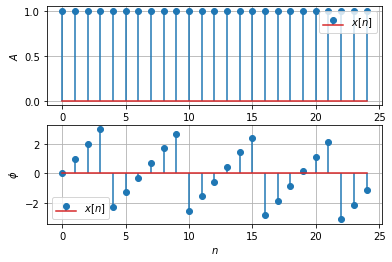
\includegraphics[width=\columnwidth]{Fig1.png}
    \caption{Input and Output Signals}
    \label{fig:plot}
\end{figure}
\end{document}
